\newcolumntype{?}{!{\vrule width 1pt}}

% \newcommand\sfac{0.082}
% \newcommand\spacercomp{4mm}
\begin{figure*}[ht!]
    \centering
    \setkeys{Gin}{width=\linewidth}
    \renewcommand\tabularxcolumn[1]{>{\Centering}m{\sfac\linewidth}} % set all columns to be centered v & hwise, with a fixed length
    \newcolumntype{D}{ >{\centering\arraybackslash} m{\imgwidthcomp} }
    \newcolumntype{E}{ >{\centering\arraybackslash} m{\labelwidthcomp} }

    % \begin{tabularx}{\textwidth}{c*{5}{X}@{\hspace{\spacercomp}}*{5}{X}c}
    % \begin{tabularx}{\textwidth}{c*{5}{X}}
    \begin{tabularx}{\textwidth}{EDDDDD}
      \textbf{Ours} &
      \includegraphics{ours_sup/n02086646-Blenheim_spaniel/orig/n02086646_1476.jpg} &
      \includegraphics{ours_sup/n02086646-Blenheim_spaniel/fit/n02086646_1476.jpg} &
      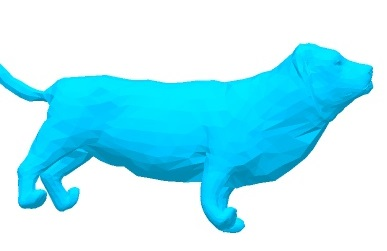
\includegraphics{ours_sup/n02086646-Blenheim_spaniel/model/n02086646_1476_crop.jpg} &
      \includegraphics{ours_sup/n02086646-Blenheim_spaniel/joints/n02086646_1476.jpg} &
      \includegraphics{ours_sup/n02086646-Blenheim_spaniel/segs/n02086646_1476.jpg} \\
      

      3D-M &
      \includegraphics{comp_sup/smal/n02086646-Blenheim_spaniel/orig/n02086646_1476.jpg} &
      \includegraphics{comp_sup/smal/n02086646-Blenheim_spaniel/fit/n02086646_1476.jpg} &
      \includegraphics{comp_sup/smal/n02086646-Blenheim_spaniel/model/n02086646_1476_fixed_crop.jpg} &
      \includegraphics{comp_sup/smal/n02086646-Blenheim_spaniel/joints/n02086646_1476.jpg} &
      \includegraphics{comp_sup/smal/n02086646-Blenheim_spaniel/segs/n02086646_1476.jpg} \\
      

      CGAS &
      \includegraphics{comp_sup/cgas/n02086646-Blenheim_spaniel/orig/n02086646_1476.jpg} &
      \includegraphics{comp_sup/cgas/n02086646-Blenheim_spaniel/fit/n02086646_1476.jpg} &
      \includegraphics{comp_sup/cgas/n02086646-Blenheim_spaniel/model/n02086646_1476_fixed_crop.jpg} &
      \includegraphics{comp_sup/cgas/n02086646-Blenheim_spaniel/joints/n02086646_1476.jpg} &
      \includegraphics{comp_sup/cgas/n02086646-Blenheim_spaniel/segs/n02086646_1476.jpg} \\
      %\hspace{\spacercomp}
     
      \textbf{Ours} &
      \includegraphics{ours_sup/n02087394-Rhodesian_ridgeback/orig/n02087394_831.jpg} &
      \includegraphics{ours_sup/n02087394-Rhodesian_ridgeback/fit/n02087394_831.jpg} &
      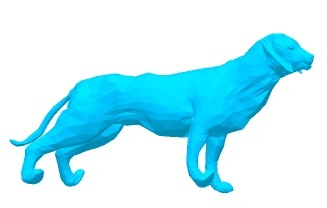
\includegraphics{ours_sup/n02087394-Rhodesian_ridgeback/model/n02087394_831_crop.jpg} &
      \includegraphics{ours_sup/n02087394-Rhodesian_ridgeback/joints/n02087394_831.jpg} &
      \includegraphics{ours_sup/n02087394-Rhodesian_ridgeback/segs/n02087394_831.jpg} \\

      3D-M &
      %\hspace{\spacercomp}
      \includegraphics{comp_sup/smal/n02087394-Rhodesian_ridgeback/orig/n02087394_831.jpg} &
      \includegraphics{comp_sup/smal/n02087394-Rhodesian_ridgeback/fit/n02087394_831.jpg} &
      \includegraphics{comp_sup/smal/n02087394-Rhodesian_ridgeback/model/n02087394_831_fixed_crop.jpg} &
      \includegraphics{comp_sup/smal/n02087394-Rhodesian_ridgeback/joints/n02087394_831.jpg} &
      \includegraphics{comp_sup/smal/n02087394-Rhodesian_ridgeback/segs/n02087394_831.jpg} \\

      CGAS &
      \includegraphics{comp_sup/cgas/n02087394-Rhodesian_ridgeback/orig/n02087394_831.jpg} &
      \includegraphics{comp_sup/cgas/n02087394-Rhodesian_ridgeback/fit/n02087394_831.jpg} &
      \includegraphics{comp_sup/cgas/n02087394-Rhodesian_ridgeback/model/n02087394_831_fixed_crop.jpg} &
      \includegraphics{comp_sup/cgas/n02087394-Rhodesian_ridgeback/joints/n02087394_831.jpg} &
      \includegraphics{comp_sup/cgas/n02087394-Rhodesian_ridgeback/segs/n02087394_831.jpg} \\
      
      % & 
      & (a) & (b) & (c) & (d) & (e) \\
      %\hspace{\spacercomp} 
      % (a) & (b) & (c) & (d) & (e) \\
    \end{tabularx}
    %
    \caption{%
    \textbf{Qualitiative comparison to SOTA.} 
    Row 1: \textbf{Ours}, 
    Row 2: 3D-M~\cite{zuffi2017menagerie}, 
    Row 3: CGAS~\cite{biggs2018creatures}. 
    (a) input image, (b) predicted 3D mesh, (c) canonical view 3D mesh, 
    (d) reprojected model joints and (e) silhouette reprojection error. 
    }
    \label{fig:comparison_1}
\end{figure*}
